\documentclass[../main.tex]{subfiles}
\begin{document}
\chapter{GameObject dan Komponen Unity}

\section{Transform}
Setiap \textit{GameObject} memiliki komponen \texttt{Transform} yang menyimpan posisi, rotasi, dan skala dalam ruang dunia atau lokal. \texttt{Transform} juga menentukan hierarki orang tua–anak yang memengaruhi sistem koordinat, sehingga transformasi pada induk ikut memengaruhi anak. Pemahaman relatif posisi lokal dan dunia membantu mencegah perilaku tak terduga saat menerapkan animasi dan fisika \parencite{unity-transform,unity-gameobjects}.

Operasi \texttt{Transform} sebaiknya mempertimbangkan \textit{frame rate} dan integrasi fisika agar tidak terjadi ketidakselarasan. Untuk pergerakan berbasis fisika, gunakan gaya atau kecepatan pada \texttt{Rigidbody} dan hindari mengubah \texttt{Transform} langsung, kecuali untuk penempatan awal. Praktik ini menjaga konsistensi simulasi tumbukan dan gravitasi \parencite{unity-transform}.

\section{Rigidbody dan Collider}
\texttt{Rigidbody} menambahkan dinamika fisika pada objek, memungkinkan penerapan gaya, torsi, dan pengaruh gravitasi. Bersama \texttt{Collider}, sistem ini mendukung pendeteksian tumbukan dan respons fisik sesuai material. Penyetelan massa, drag, dan kendala perlu seimbang untuk stabilitas, sementara mode deteksi tumbukan \textit{continuous} mencegah objek cepat menembus permukaan \parencite{unity-rigidbody,unity-collider}.

Perbedaan \textit{dynamic} dan \textit{kinematic} \texttt{Rigidbody} berdampak pada interaksi: objek kinematik digerakkan skrip namun tetap dapat memicu tumbukan. Collider bertipe \textit{trigger} cocok untuk deteksi kawasan tanpa respons fisika, sedangkan collider non-\textit{trigger} untuk tumbukan nyata. Pemilihan kombinasi harus diselaraskan dengan tujuan desain interaksi \parencite{unity-collider}.

\begin{table}[h]
  \centering
  \caption{Perbandingan tipe \texttt{Rigidbody} dan penggunaan collider}
  \begin{tabularx}{\textwidth}{@{}lXX@{}}
    \toprule
    Tipe & Karakteristik & Kasus Penggunaan \\
    \midrule
    Dynamic & Dipengaruhi gaya dan gravitasi & Objek fisik interaktif (peti, proyektil) \\
    Kinematic & Dikendalikan skrip, tidak dipengaruhi gaya & Pintu geser, platform bergerak \\
    Trigger Collider & Tidak ada respons fisika, memicu event & Zona pickup, deteksi area \\
    \bottomrule
  \end{tabularx}
\end{table}

\section{Prefab}
\textit{Prefab} menyediakan cetak biru objek untuk instansiasi ulang yang konsisten di berbagai adegan. Dengan menyimpan konfigurasi komponen sebagai aset, pembaruan pada definisi utama akan mengalir ke seluruh instans. Fitur varian dan override memungkinkan kustomisasi sambil mempertahankan hubungan ke definisi dasar \parencite{unity-prefab}.

Arsitektur berbasis prefab mendorong modularitas dan pengujian. Pemisahan logika, data, dan presentasi mengurangi dampak perubahan silang, sementara konvensi penamaan dan struktur folder yang rapi mempercepat pencarian aset. Dokumentasi pola penggunaan prefab di tim membantu mengurangi regresi saat iterasi \parencite{unity-prefab,unity-project-structure}.

\begin{figure}[h]
  \centering
  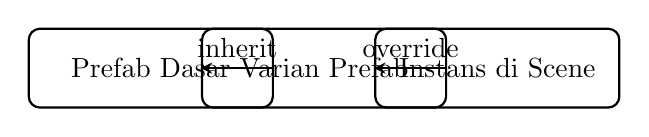
\begin{tikzpicture}[node distance=2.2cm,>=stealth,thick]
    \tikzstyle{nodeA}=[rectangle, draw, rounded corners, minimum width=3.1cm, minimum height=1cm, align=center]
    \node[nodeA] (base) {Prefab Dasar};
    \node[nodeA, right of=base] (variant) {Varian Prefab};
    \node[nodeA, right of=variant] (instance) {Instans di Scene};
    \draw[->] (base) -- node[above]{inherit} (variant);
    \draw[->] (variant) -- node[above]{override} (instance);
  \end{tikzpicture}
  \caption{Relasi prefab dasar, varian, dan instans di scene \parencite{unity-prefab}.}
\end{figure}

\onlyinsubfile{\printbibliography}
\end{document}
